\subsection{Standard Model QCD Multijet}
\label{sec:Bkg:QCD}

\indent  QCD multijet events form a significant contribution to background rates in signal region bins with $\RISR < 0.4$.  The QCD multijet process creates little intrinsic $\met$ from actual neutrinos. Instead, misreconstructed jets are the primary reason why some QCD multijet events are able to pass the $\met > 250 \gev$ requirement and the signal region selections.  Misreconstructed jets can cause an imbalance in the total event $E_t$ and lead to events with a large reconstructed $\met$ even if the event has little intrinsic $\met$.  We estimated the QCD background using the data driven {\tt Jet Smearing} method.   \\

\subsubsection{The {\tt Jet Smearing} Method of Estimating QCD Background}

\indent The {\tt Jet Smearing} method first selects seed events from data with well reconstructed jets and little $\met$.  We then repeatedly smear the seed events' jets with a predetermined jet energy response.  The resulting {\tt pesudo-data} events can have potentially large $\met$ due to the smeared jets.  A schematic demonstrating the {\tt jet smearing} method is shown in Figure \ref{fig:jetsmearing}.\\

\begin{figure}[h!]
\begin{center}
\includegraphics[width=0.45\textwidth]{figures/QCDJetSmearing/jet_smearing.pdf}
\end{center}
\caption[Schematic diagram demonstrating the {\tt Jet Smearing} method of estimating QCD background]{Schematic diagram demonstrating the {\tt Jet Smearing} method of estimating rate of QCD background.  Seed events with good jet energy measurements are repeatedly smeared with predetermined jet energy resolutions.  The new $\met$ is calculated as the difference between the seed event's and smeared event's jet momentum plus the original seed event's $\met$.\cite{JetSmearing} }
\label{fig:jetsmearing}
\end{figure}

\indent The {\tt Jet Smearing} methods have a number of inherent assumptions about the generation of $\met$ in QCD multijet background.  These assumptions include: \\

\begin{itemize}
\item The jet response captures all sources of jet $\pt$ measurement fluctuations
\item The $\met$ in multijet events result predominately from mis-measured jets
\item Jet response is independent on the presence of other jets and jet smearing can be applied on a jet-by-jet basis
\end{itemize}

\indent These assumptions seem to be well satisfied in the high $\met$, high jet multiplicity environment of the signal region.  Other sources of $\met$ not taken into account by the jet smearing method such as $\met$ from pileup jets, mis-reconstructed soft term of the $\met$ and object overlap removal are assumed to be negligible in the signal region. \\

\indent We then define a QCD control region that is kinematic similar to the signal region but dominated by QCD background.  We normalize the predicted QCD rate to the amount of data in the control region.  The normalization factor is then applied to predicted QCD rates in the signal region.  We also validate the QCD predictions using a QCD validation region.  The QCD control and validation regions are covered in greater details in section \ref{sec:QCD:CR}. \\

\subsubsection{{\tt Jet Smearing} Seed Event Selection and Jet Response Function}

\indent We select for events with multiple well reconstructed jets and no leptons as seed events.  Because QCD multijet events have low intrinsic $\met$, seed events must have low $\met$ relative to the total reconstructed $E_T$ in the event. \\ 

\indent Some $\met$ is expected even in well reconstructed multijet events because both the electromagnetic and hadronic calorimeters at ATLAS are sampling calorimeters.  The energy deposited in the absorber material is effectively lost because the absorber does not actively record a signal.  Therefore the energy measured using the active material must be scaled up to compensate for this loss.  The statistical nature of the sampling process means the uncertainty, $\sigma E_T$, for jets depend on the total $E_T$.   \\

\indent The quantity $\met\rm{sig.}=\frac{ \met-8\rm{\,GeV} } {\sum E_\mathrm{T} }$ measures the significance of $\met$ relative to total hadronic activity in an event.  An event with low $\met\rm{sig.}$ has a low amount of $E_T$ imbalance relative to the total amount of calorimeter activity in the event.  In this case, the amount of $E_T$ imbalance is consistent with the expected uncertainty on calorimeter energy measurements.  If $\met\rm{sig.}$ is high then the $\met$ is inconsistent with the expected uncertainty on calorimeter measurements and the probability of having energetic weakly interacting particles in the event is high.   \\

\indent QCD multijet events are expected to produce very few energetic neutrinos and therefore, we select for well reconstructed seed events by requiring low $\met\rm{sig.}$. Seed events are selected according to the criteria listed in Table \ref{tb:seed_events_presel}. \\

 \begin{table}[h!]
 \begin{center}
 \begin{tabular}{c} \hline
   Selection \\ \hline
   $n_\mathrm{prim. vertices} > 0$\\
   Jet trigger\\
   Bad jet veto\\
   Cosmic muon veto\\
   Bad muon veto\\
   {\tt Baseline} lepton veto\\
   $\geq 4$ jets\\
   $\geq 1$ $b$-jets\\
   $\met\rm{sig.} < 0.3 + 0.1\cdot n_{\textup{n-bjets}}$ \\ \hline
 \end{tabular}
 \end{center}
 \caption{{\tt Jet Smearing} seed event preselection}
 \label{tb:seed_events_presel}
 \end{table}

\indent The $\met\rm{sig.} < 0.3 + 0.1\cdot n_{\textup{n-bjets}}$ requirement depends on the number of b-jets because b-quarks can emit significant portions of their energy in the form of neutrinos.  We therefore expect larger $\met\rm{sig.}$ in events with more b-jets.  B-jets also have a different jet response function than light quark jets to account for this effect. \\

\indent The jet response function used in {\tt Jet Smearing} includes contributions from the following effects: \\

\begin{itemize}
\item Limited calorimeter granularity
\item Hadronic energy falling outside of the jet radius or failing to be clustered correctly by jet reconstruction.
\item Additional energy clustered into the jet that results from other sources.
\item Energetic jet punching through the calorimeter.
\item Dead material in the calorimeter.
\item b-quark generating real $\met$ through decay to neutrinos.  
\end{itemize}

\subsubsection{QCD multijet Control Region and Validation Region}
\label{sec:QCD:CR}

\indent The QCD control region is designed to be similar to the signal region except the $\mindphijettwomet$ is required to be between $0.05$ to $0.1$ instead of greater than $0.04$.  $\mindphijettwomet$ is defined in equation \ref{eqn:dphijetmet} as the separation in $\phi$  between $\met$ and the two highest $\pt$ jets in the event.  \\

\indent If the $\met$ mainly results from a single misreconstructed energetic jet then we would expect the $\met$ and jet to be collinear in $\phi$.  The $\mindphijettwomet > 0.4$ selection rejects such events in the signal region.  The QCD control region selects for events with $0.05 < \mindphijettwomet < 0.1$ which is dominated by QCD.  \\

\begin{equation}
\dphijettwomet = \min_{2~highest~pt~jets} \Delta \phi ( jet, \met ) 
\label{eqn:dphijetmet}
\end{equation}

%This region is dominated by QCD backgrounds with high $\met$ due to a single mis-reconstructed energetic jet but with the same jet multiplicity and jet kinematics required in the signal region. \\

\indent The pseudo-data resulting from the {\tt Jet Smearing} processes is then normalized to data using the QCD control region defined in Table \ref{tab:QCDCR}.  

\begin{table}[h!]
  \begin{center}
    \def\arraystretch{1.4}%
    \begin{tabular}{c|c} \hline\hline
      {\bf Variable} &  QCD control region  \\ \hline \hline
      \mindphijettwomet  & [0.05,0.1]  \\  
      \nBJetS & {$\ge1$} \\
      \nJetS & {$\ge5$}  \\
      \pTISR & $>150$ GeV   \\
      \pTSBZero &{$>40\gev$}  \\
      \pTSFour & {$>50$ GeV}   \\
      \dPhiISRMET &  $>2.00$  \\ 
      \rISR  & {$<0.4$} \\ \hline \hline
    \end{tabular}
  \caption{QCD control region selections, in addition to the zero lepton preselection in Table~\ref{tab:0Lcommon}. }
     \label{tab:QCDCR}
  \end{center}
\end{table}%

\indent Data vs QCD pseudo-data distributions for the $\PTISR$, $\dphiISRI$ and $\MS$ variables in the QCD control region can be seen in Figure \ref{fig:QCD:CR}.  We extrapolate over these variables between the control and signal regions. \\

\begin{figure}[!h]
\begin{center}
    \begin{subfigure}[b]{0.40\textwidth}  
    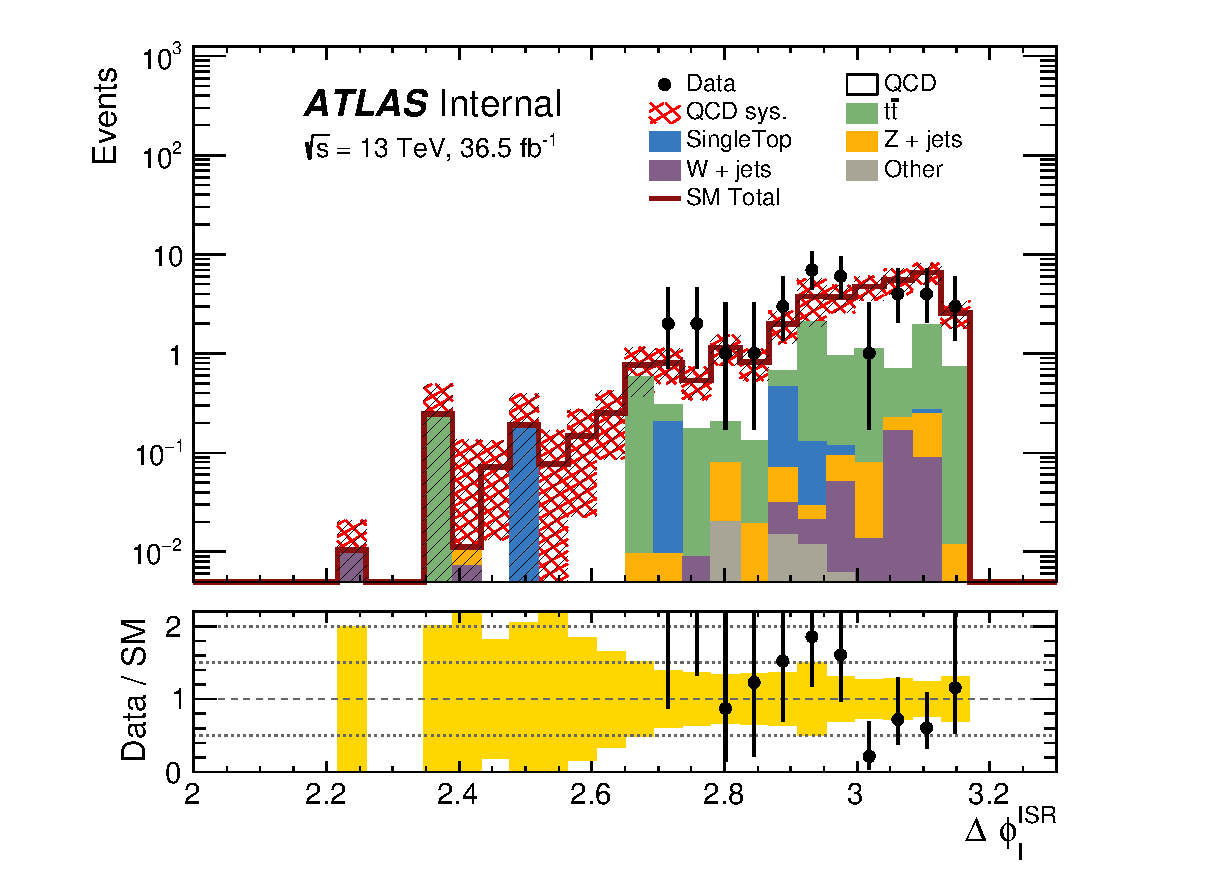
\includegraphics[width=\textwidth]{figures/QCDJetSmearing/CRQC/dphiISRI_36500.eps}
                \caption{ }
    \end{subfigure}
    \begin{subfigure}[b]{0.40\textwidth}  
    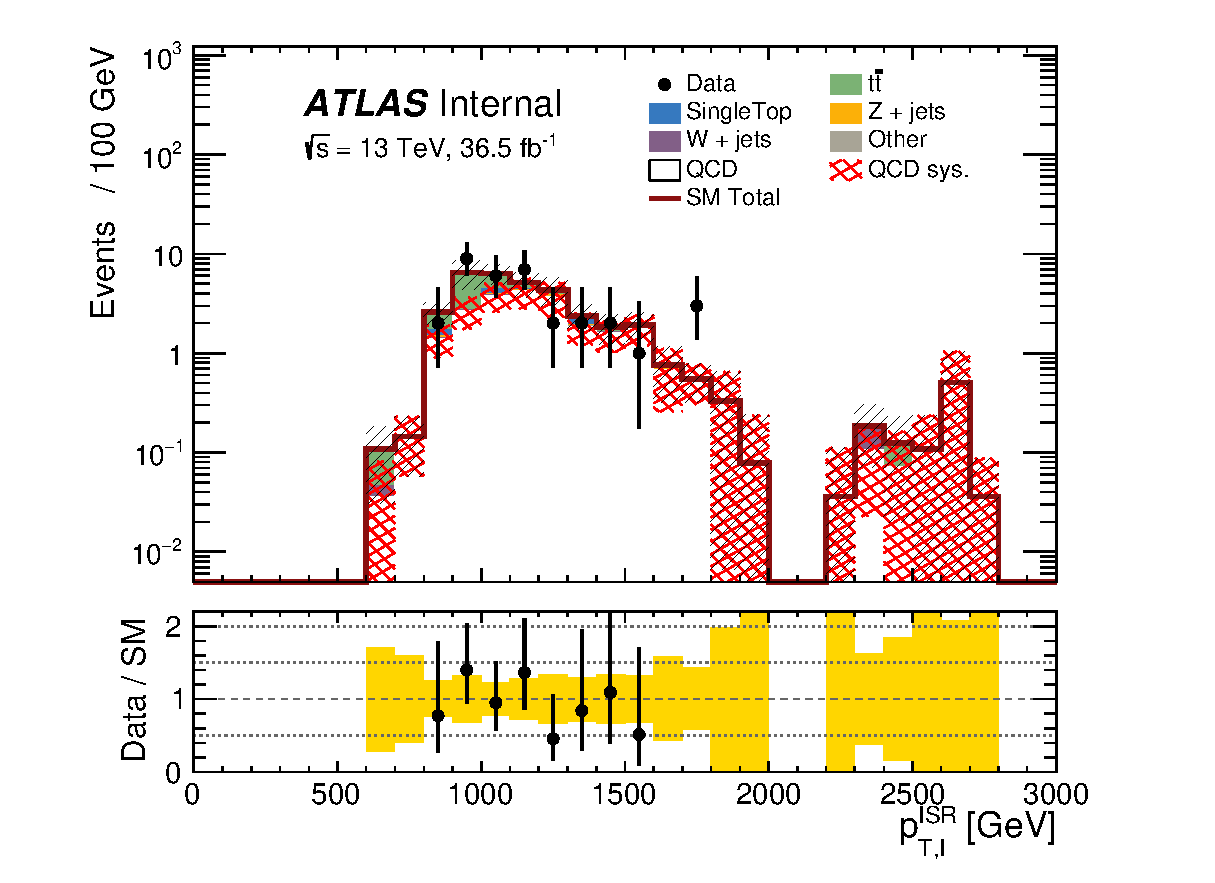
\includegraphics[width=\textwidth]{figures/QCDJetSmearing/CRQC/PTISR_36500}
                \caption{ }
    \end{subfigure}
        \begin{subfigure}[b]{0.40\textwidth}  
    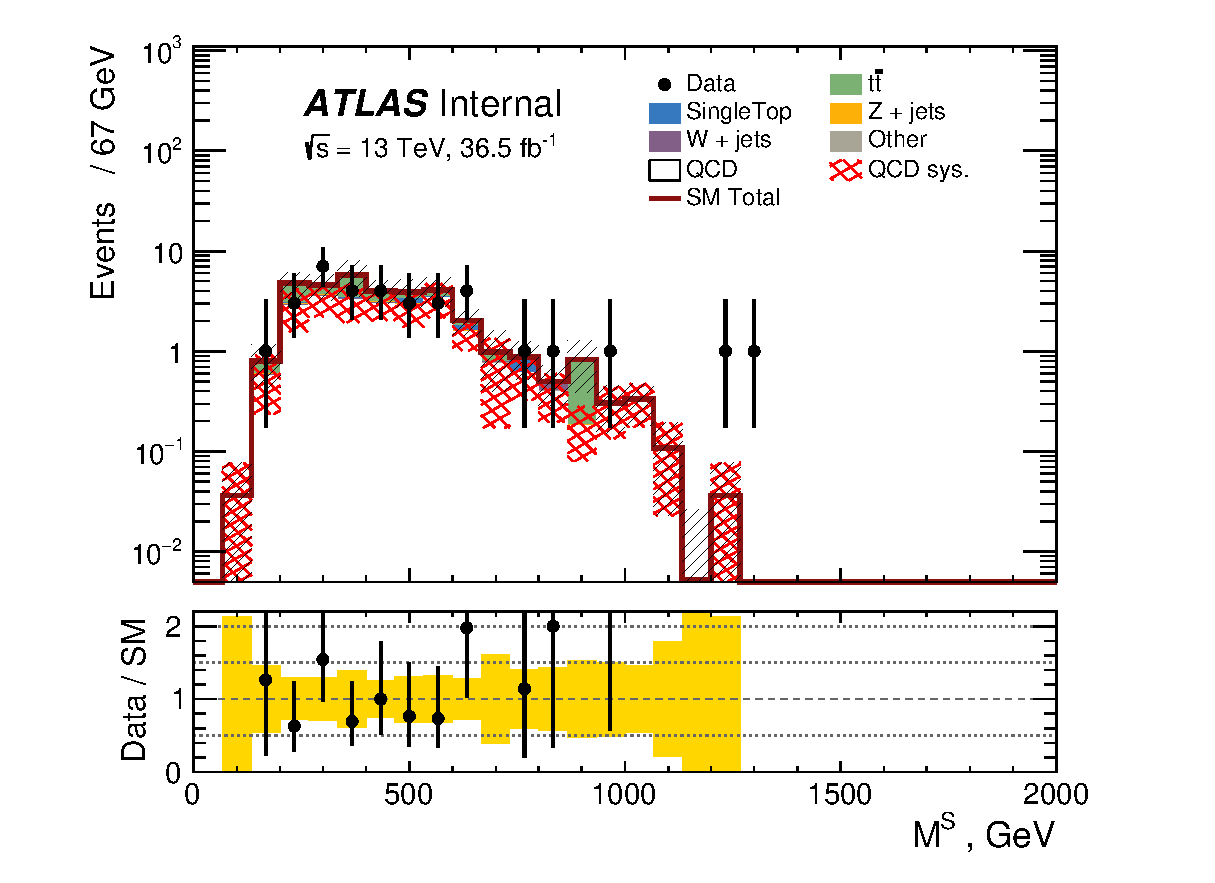
\includegraphics[width=\textwidth]{figures/QCDJetSmearing/CRQC/MV_36500}
                    \caption{ }
    \end{subfigure}
\caption[$\PTISR$, $\dphiISRI$ and $\MS$ distributions in the QCD control region]{$\PTISR$, $\dphiISRI$ and $\MS$ distributions in the QCD control region}
\label{fig:QCD:CR}
\end{center}
\end{figure}

\indent The QCD multijet prediction after normalizing to the control region can be checked in the QCD validation region defined in Table \ref{tab:QCDVR}.   The QCD validation region has the exact same kinematic selection as the signal region except a lower $\mindphijettwomet$ requirement of between $0.1$ and $0.2$.  $\RISR$ is also required to be below $0.4$ as we don't expect significant QCD contribution at higher $\RISR$.  \\

\begin{table}[h!]
  \begin{center}
    \def\arraystretch{1.4}%
    \begin{tabular}{c|c} \hline\hline
      {\bf Variable} &  QCD Validation Region  \\ \hline \hline
      \mindphijettwomet  &  [0.1,0.2]           \\  
      \nBJetS & $\ge1$ \\
      \nJetS & $\ge5$  \\
      \pTISR & $>400$ GeV \\ 
      \pTSBZero & $>40\gev$  \\ 
      \pTSFour & $>50$ GeV  \\
      \mS & $>300\gev$  \\
      \dPhiISRMET &  $>3.00$  \\ 
      \rISR  & $<0.4$ \\ \hline \hline
    \end{tabular}
  \end{center}
  \caption{QCD validation region selections, in addition to the zero lepton preselection in Table~\ref{tab:0Lcommon}. }
   \label{tab:QCDVR}
\end{table}%

\indent Data vs QCD pseudo-data distribution for the $\RISR$ and $\dphiISRI$ variables in the QCD validation region can be seen in Figure \ref{fig:QCD:CR}.  A good agreement is found between data and pseudo-data predictions. \\

\begin{figure}[!h]
\begin{center}
    \begin{subfigure}[b]{0.40\textwidth}  
    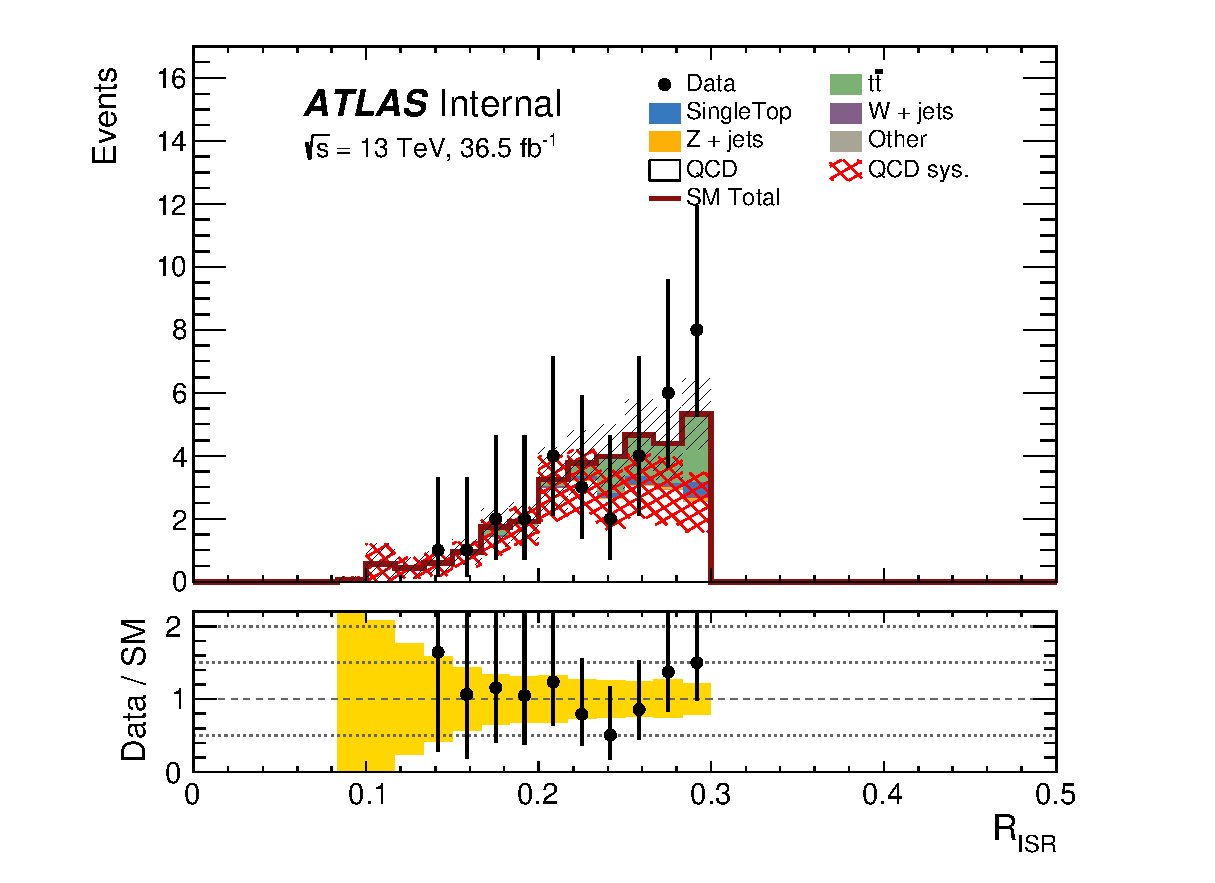
\includegraphics[width=\textwidth]{figures/QCDJetSmearing/VRqC/RISR_36500} 
                \caption{ }
    \end{subfigure}
    \begin{subfigure}[b]{0.40\textwidth}  
    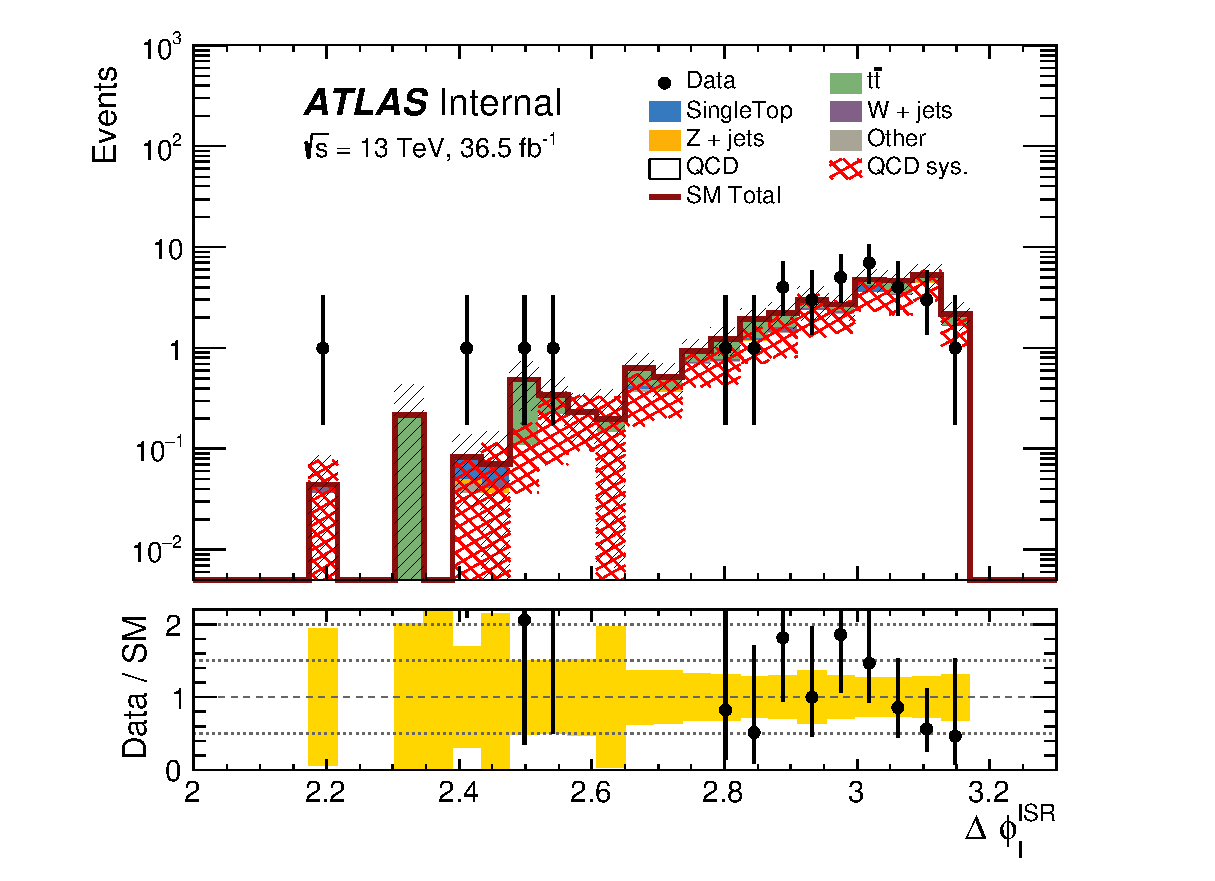
\includegraphics[width=\textwidth]{figures/QCDJetSmearing/VRqC/dphiISRI_36500.eps}
                \caption{ }
    \end{subfigure}
\caption[$\RISR$ and $\dphiISRI$ distributions in the QCD validation regions]{$\RISR$ and $\dphiISRI$ distributions in the QCD validation region.}
\label{fig:QCD:VR}
\end{center}
\end{figure}

\subsubsection{QCD prediction in the Signal Region}

\indent The predicted amount of QCD in the signal region is given by the amount of QCD pseudo-data that pass the signal region selections after normalizing to the QCD control region. The systematic uncertainty on the signal region QCD prediction is given by repeating the {\tt Jet Smearing} process with a tighter and looser set of seed event selections.  \\

\indent An upward error corresponds to using seed events requiring $\met\rm{sig.} < 0.6 + 0.2\cdot n_{\textup{n-bjets}}$ and an lower error corresponds to using seed events requiring $\met\rm{sig.} < 0.2 + 0.05\cdot n_{\textup{n-bjets}}$. QCD multijet events with better reconstructed jets tend to have a smaller $\met\rm{sig.}$. \\

\indent The expected QCD yield and uncertainty in the signal region is given in Table \ref{tab:QCDYields}.\\

\begin{table}[!h]
  \begin{center}
    \begin{tabular}{c|c|c|c} \hline\hline
SR $\RISR$ Region       & 0.3-0.4              & 0.4-0.5              & 0.5-0.6              \\ \hline
QCD expected yield & $4.56\pm2.38$ & $1.58\pm0.77$ & $0.32\pm0.17$  \\ \hline \hline
    \end{tabular}
        \begin{tabular}{c|c|c} \hline\hline
SR $\RISR$ Region         & 0.6-0.7             & 0.7-0.8 \\ \hline
QCD expected yield       & $0.04\pm0.02$ & $0.00\pm0.00$ \\ \hline \hline
    \end{tabular}
  \caption{Expected yields of the QCD multijet backgrounds in the signal region.}
  \label{tab:QCDYields}
  \end{center}
\end{table}%
